% This must be in the first 5 lines to tell arXiv to use pdfLaTeX, which is strongly recommended.
\pdfoutput=1
% In particular, the hyperref package requires pdfLaTeX in order to break URLs across lines.

\documentclass[11pt]{article}

% Remove the "review" option to generate the final version.
\usepackage{main}

% Standard package includes
\usepackage{times}
\usepackage{latexsym}

% \usepackage{hyperref}
% \usepackage{glossaries}
% \usepackage{latexsym}

\makeatletter
\newcommand{\printfnsymbol}[1]{%
  \textsuperscript{\@fnsymbol{#1}}%
}
\makeatother

% For proper rendering and hyphenation of words containing Latin characters (including in bib files)
\usepackage[T1]{fontenc}
% For Vietnamese characters
% \usepackage[T5]{fontenc}
% See https://www.latex-project.org/help/documentation/encguide.pdf for other character sets

% This assumes your files are encoded as UTF8
\usepackage[utf8]{inputenc}

% This is not strictly necessary, and may be commented out.
% However, it will improve the layout of the manuscript,
% and will typically save some space.
\usepackage{microtype}

% This is also not strictly necessary, and may be commented out.
% However, it will improve the aesthetics of text in
% the typewriter font.
\usepackage{inconsolata}


% my package
\usepackage{amsmath}
\usepackage{amssymb}
\usepackage[capitalise]{cleveref}
% \usepackage{lipsum}
\usepackage{blindtext}
\usepackage{graphicx}
\usepackage{multirow}
\usepackage{booktabs}
\usepackage{subfigure}
\usepackage{stfloats}

\usepackage{paralist}
\usepackage[shortlabels]{enumitem}

\usepackage{xspace}
\newcommand*{\eg}{e.g.\@\xspace}
\newcommand*{\ie}{i.e.\@\xspace}

\newcommand{\ModelName}{EMAT\xspace}
\newcommand{\ModelNames}{EMATs\xspace}
\newcommand{\MemoryName}{AAMA\xspace}

% 
\newcommand{\exper}[1]{\textsc{#1}}
\newcommand{\prefix}{\exper{Prefix}\xspace}

\DeclareMathOperator*{\argmax}{arg\,max}
\DeclareMathOperator*{\argmin}{arg\,min}
% \DeclareMathOperator{\E}{\mathbb{E}}

%\newcommand{\eg}{e.g.,}
%\newcommand{\ie}{i.e.,}

% Acronyms
\usepackage{glossaries}
\glsdisablehyper
\newacronym{ODQA}{ODQA}{Open-Domain Question Answering}


\newif\ifcomments
% Comment out to disable all in-line comments.
% \commentstrue

\newcounter{psCounter}
\newif\ifpsvar
\ifcomments
    \psvartrue
\fi
\ifpsvar
    \newcommand{\ps}[1]{{\small \color{red} \refstepcounter{psCounter}\textsf{[PS]$_{\arabic{psCounter}}$:{#1}}}}
\else
    \newcommand{\ps}[1]{}
\fi

\newcounter{ywCounter}
\newif\ifywvar
\ifcomments
    \ywvartrue
\fi
\ifpsvar
    \newcommand{\yw}[1]{{\small \color{cyan} \refstepcounter{ywCounter}\textsf{[YW]$_{\arabic{ywCounter}}$:{#1}}}}
\else
    \newcommand{\yw}[1]{}
\fi

\newcounter{pmmCounter}
\newif\ifywvar
\ifcomments
    \ywvartrue
\fi
\ifpsvar
    \newcommand{\pmm}[1]{{\small \color{red} \refstepcounter{pmmCounter}\textsf{[PM]$_{\arabic{pmmCounter}}$:{#1}}}}
\else
    \newcommand{\pmm}[1]{}
\fi

\title{Retrieval-Augmented Generation for Enhancing Open-Domain Question Answering Systems with External Knowledge}

\author{
  Zhuo Chen \\
  University of California, Berkeley \\
  { \normalsize \tt  zhuochen@berkeley.edu} \\
}

\begin{document}
\maketitle

\begin{abstract}
This paper investigates the impact of retrieval-augmented generation on the performance of large language models (LLMs) in Open-Domain Question Answering (ODQA). We incorporate an external knowledge augmentation system leveraging the PAQ dataset, which enriches LLMs like Flan-T5 and Llama-2-13B-chat with real-time access to over 1.4 million question-answer pairs. By enabling dynamic retrieval of relevant information, we aim to overcome the inherent limitations of LLMs related to fixed knowledge bases and context length constraints. The study evaluates enhancements in accuracy, employing metrics such as Exact Match, F1, and Rouge scores. Our results demonstrate that retrieval-augmented techniques significantly improve the answer quality across various LLMs (\eg, $8.45 \rightarrow 35.48$ EM on Flan-T5-large), highlighting the potential of integrating these systems to extend the capabilities and applicability of traditional neural language models in complex question answering tasks.\footnote{Code and datasets are available at \url{https://github.com/chenzhuo1005/datasci-w266-nlp-project}.}
\end{abstract}

\section{Introduction}

The emergence of ChatGPT and the widespread use of transformer based large-language-models (LLMs) have significantly improved many areas of NLP tasks. LLMs can converse, answer questions, reason logically, and retrieve information from its parametric stored human knowledge. Despite its impressive capabilities, LLMs such as GPTs series have notable limitations. First, it is restricted by context length, with \emph{GPT-3.5-Turbo-0613} supporting a 4096-token window~\cite{gpt3.5turbo} and \emph{GPT-4-0613} supporting an 8192-token window~\cite{gpt4turbo}. This limitation affects the model's ability to understand and remember longer text contexts. Second, LLMs are trained through pretraining and fine-tuning, which compresses knowledge into the model's parameters. Studies show that these models capture only partial knowledge~(\citet{LAMA}), and while increasing the model size can improve coverage~\citep{T5,DBLP:conf/emnlp/RobertsRS20,GPT3}, it requires more computational resources and time. Lastly, the models are limited by their knowledge cutoff, with both \emph{GPT-3.5-Turbo-0613} and \emph{GPT-4-0613}'s knowledge being up-to-date only until September 2021~\cite{gpt3.5turbo, gpt4turbo}. Updating the models to include the latest knowledge requires retraining and releasing newer versions, and the stored knowledge may not cover new or unseen data, especially in specific expert domains, leading to potential inaccuracies and hallucinations~\cite{maynez-etal-2020-faithfulness}.

In addition to encoding knowledge directly into model parameters, \emph{retrieval-augmented models}~\citep{REALM, RAG, FiD, spanlp-2022-semiparametric}, can access external sources like Wikipedia and retrieve relevant information and incorporate it into LLM’s output generation process. \cref{fig:arch} shows general workflows of \emph{retrieval-augmented generations}. This approach has significantly improved the accuracy of answering open-domain questions, where the model must respond without specific context~\citep{DBLP:conf/acl/ChenFWB17}. Furthermore, RAG can be tailored to specialized fields by creating domain-specific knowledge embeddings. These embeddings are stored in vector databases and can be retrieved based on queries, enriching the model's context for more accurate responses.

To explore the potential of retrieval-augmented approaches to enhance the Open-Domain Question Answering (ODQA) task of large language models, this study devises an external knowledge augmentation system. This system incorporates approximately 14 million Question-Answer pairs sourced from the \emph{PAQ} dataset~\citep{paq}, a large collection of question-answering generated from Wikipedia, as the system’s knowledge source. Utilizing the \emph{LlamaIndex} APIs, key-value embeddings for each Question-Answer pair were generated and stored within \emph{Pinecone}, a managed vector database service renowned for vector similarity search. The evaluation process uses the \emph{nq\_open}~\citep{doi:10.1162/tacl-a-00276, lee-etal-2019-latent} validation dataset, an open domain question answering benchmark that is derived from Natural Questions~\citep{lee-etal-2019-latent}. For the inference tasks pertaining to question answering, this study employs a selection of large language models: \emph{Flan-T5-base}, \emph{Flan-T5-large}, \emph{Llama-2-13B-chat}, and \emph{GPT-3.5-Turbo}, comparing the standard versions of these models with versions enhanced by \emph{PAQ} dataset knowledge. Performance is measured using \emph{Exact Match (EM)}, \emph{F1}, and \emph{Rouge scores} to evaluate the effectiveness of knowledge augmentation.


\begin{figure*}[t]
\begin{center}
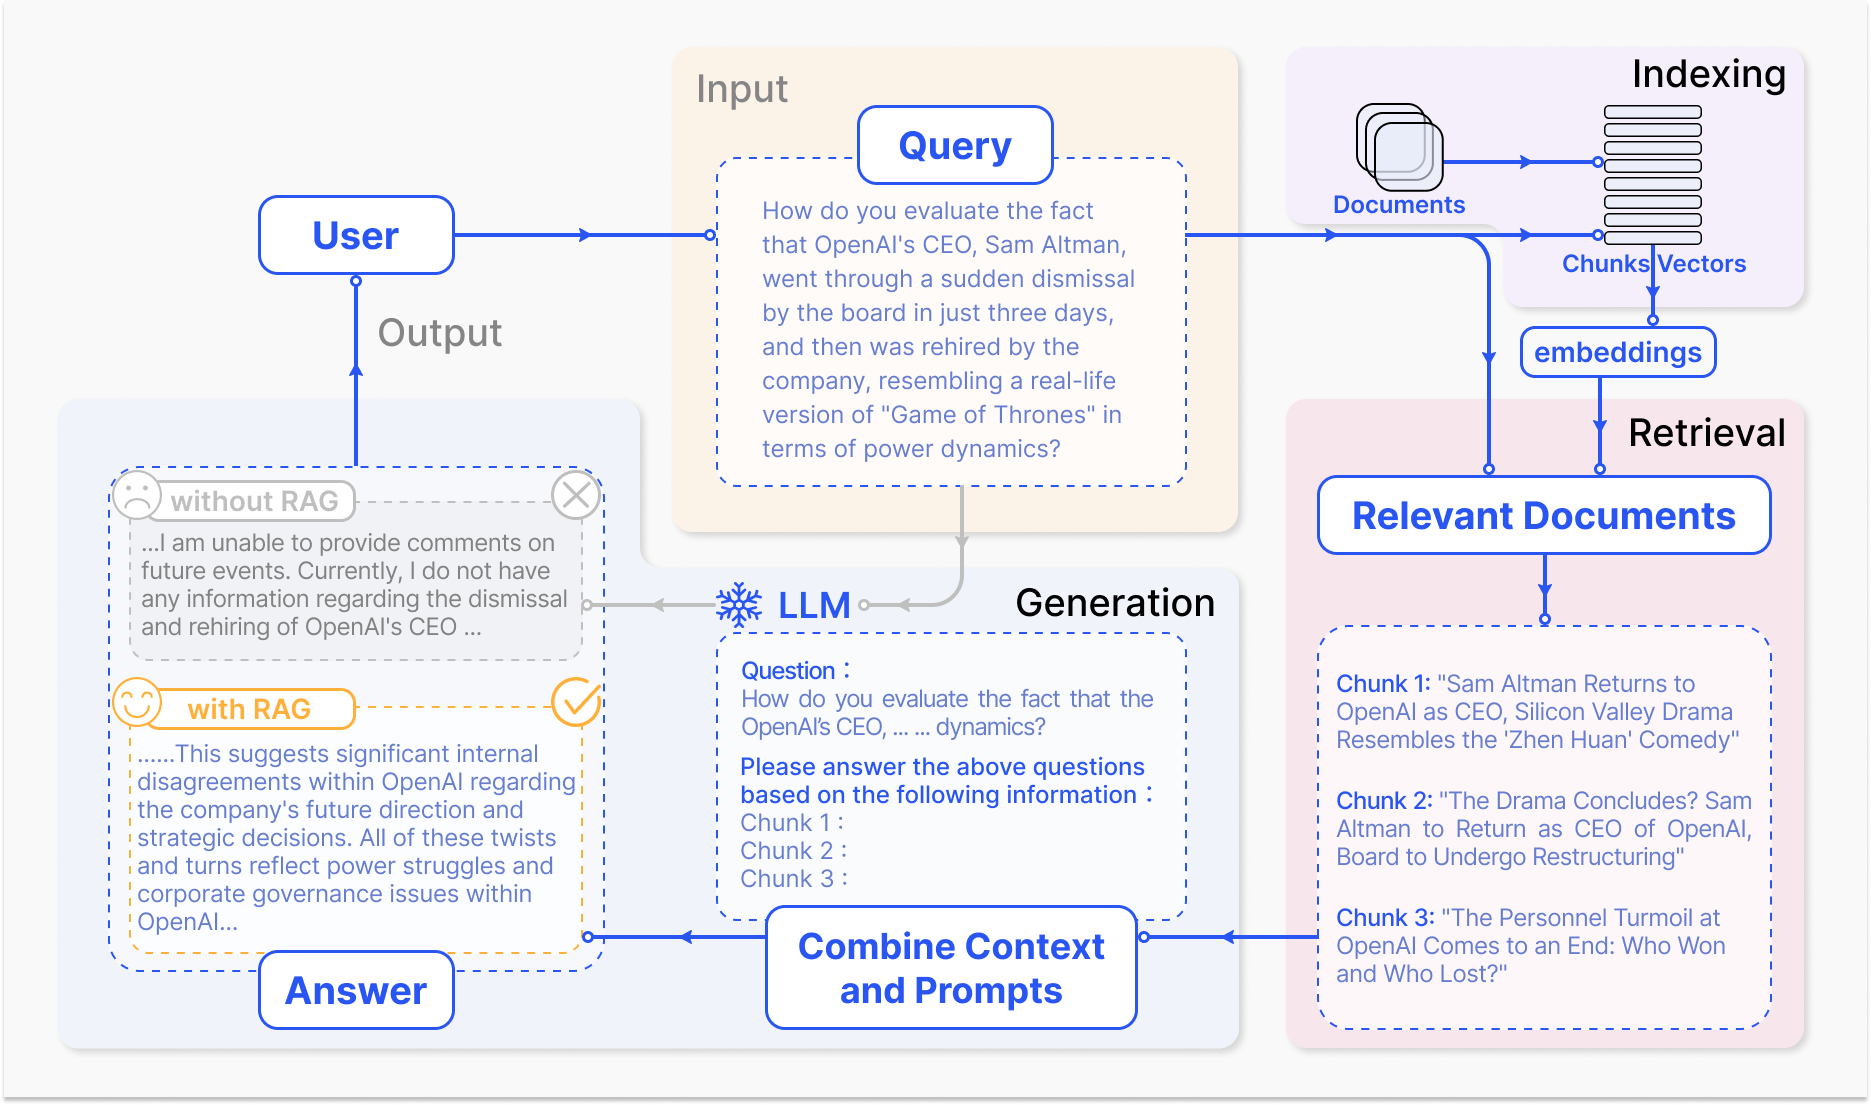
\includegraphics[width=0.9\textwidth]{images/RAG_case.png}
\end{center}
\caption{
Architecture of Retrieval-Augmented Generation (RAG)~\citep{gao2024retrievalaugmented}: factual knowledge is stored in a key-value memory where keys and values correspond to questions and answers, respectively;
during inference, the model retrieves information from the memory via similarity search and uses it to condition the generation process.
}
\label{fig:arch}
\end{figure*}

\section{Project Overview}

\subsection{Datasets}

The dataset utilized in this study is the \emph{nq\_open} validation dataset, hosted on HuggingFace (\url{https://huggingface.co/datasets/nq_open/viewer/nq_open/validation}). This validation dataset, introduced by~\citep{lee-etal-2019-latent}, comprises 3,610 question-answer pairs and serves as a benchmark for open-domain question answering, derived from \emph{NaturalQuestions}. The objective is to predict an English answer string for a given English question.

\subsection{Knowledge Source}

The \emph{PAQ} dataset~\citep{paq} serves as the knowledge source and is available on GitHub (\url{https://github.com/facebookresearch/PAQ?tab=readme-ov-file#paq-qa-pairs}). The QA pairs in PAQ were trained and retrieved from \emph{NaturalQuestions} and \emph{TriviaQA}, with the full version containing 64.9M QA pairs. For this project, We utilized \emph{PAQ-L1}, a lighter version of \emph{PAQ} with 14.1M QA pairs. Although \emph{PAQ-L1} has more than four times fewer data rows, it still maintains substantial coverage of \emph{NQ} (88.3\%) and \emph{TQA} (90.2\%) compared to the full \emph{PAQ} version, which covers \emph{NQ} (90.2\%) and \emph{TQA} (91.1\%)~\citep{paq}. Since the \emph{PAQ} data is derived from \emph{NaturalQuestions}, it encompasses the coverage of the \emph{nq\_open} dataset mentioned earlier and is thus a suitable candidate for a knowledge source in knowledge augmentation generation.

\begin{table}
\renewcommand\arraystretch{1.2} 
\setlength\tabcolsep{4pt}
\centering
\resizebox{\columnwidth}{!}{
    \begin{tabular}{ll}
    \toprule
    \multicolumn{2}{c}{\textbf{Natural Question (\emph{PAQ})}} \\ \midrule
    \textbf{Q}: where is conan meriadoc from? & \textbf{A}: \emph{british} \\ \midrule
    \multicolumn{2}{l}{\textbf{Retrieved Key-Values}} \\
    \textbf{Q}: who is conan meriadoc mentioned alongside in & \textbf{A}: cadwaladr \\ armes prydein? \\
    \textbf{Q}: who argued that conan meriadoc dates back to  & \textbf{A}: hubert guillotelr \\ the mid 12th century? \\
    \textbf{Q}: conan meriadoc was the roman name for whom? & \textbf{A}: magnus maximus \\
    \textbf{Q}: who is the compiler of conan meriadoc? & \textbf{A}: gurheden \\
    \textbf{Q}: what nationality was conan meriadoc? & \textbf{A}: \underline{\emph{british}} \\
    \bottomrule
    \end{tabular}
}
    \caption{Example question from \emph{PAQ} and its associated answer, along with the top-5 question-answer pairs retrieved from the vector store by similarity search.}
    \label{tab:paq_with_scores}
\end{table}

\subsection{Build Knowledge}

The process of building knowledge is crucial for knowledge retrieval and augmentation. The aim is to transform the raw \emph{PAQ-L1} data, which consists of question-answer text pairs, into key-value knowledge embeddings, using the question as the embedding key. The choice of the embedding model is also significant, as it impacts the precision of knowledge compression and retrieval, as well as the speed of embedding computation. After thorough research and considering both accuracy and efficiency, \emph{BAAI/bge-small-en}~\cite{bge_embedding} was chosen for its lower computational demand yet competitive performance. This model is based on the English language and has an embedding size of 384. Given that both the knowledge source and the evaluation dataset consist of brief questions and answers, an embedding size of 384 is deemed sufficient to encapsulate the relevant information.

Given the limited GPU computing power, a batch size of 500 for the embedding computation step has been determined. The embedded QA pairs are then stored in \emph{Pinecone} vector database and are integrated into a node retrieval object implemented by \emph{LlamaIndex} APIs. This retrieval object takes a question as the query text, computes its embedding using the same \emph{BAAI/bge-small-en} embedding model, and performs a vector similarity search in \emph{Pinecone}. The top-k embedded QA pairs are returned with their associated scores. \cref{tab:paq_with_scores} shows an example question and the top-5 retrieved answers from \emph{PAQ}.

Last, the question associated with the retrieved knowledge QA pairs with scores will be passed to LLMs for generation inference.

\subsection{Model Selection}

\emph{Flan-T5-base}: A variant of \emph{T5-base} with the same number of parameters (220 million) but has been fine-tuned on over 1,000 additional tasks~\citep{https://doi.org/10.48550/arxiv.2210.11416}. It outperforms \emph{T5-base} in many tasks, including question-answering. It has also been fine-tuned with instruction-based prompt texts, allowing it to utilize external knowledge to provide answers. Therefore, \emph{Flan-T5-base} has been selected as the baseline model. HuggingFace: \url{https://huggingface.co/google/flan-t5-base}

\vspace{0.3\baselineskip}

\noindent\emph{Flan-T5-large}: With an increased number of parameters (770 million), \emph{Flan-T5-large} retains all the features of \emph{Flan-T5-base} and represents a slight advancement over the baseline model.
HuggingFace: \url{https://huggingface.co/google/flan-t5-large} 

\vspace{0.3\baselineskip}

\noindent\emph{Llama-2-13B-chat-GGUF}: Similar to \emph{Llama-2-13B-chat-hf} except for its format, introduced by the \emph{llama.cpp} team. Llama 2 consists of a series of pretrained and fine-tuned generative text models developed by Meta~\citep{touvron2023llama}. In this study, we use the 13 billion parameter version of Llama 2, optimized for dialogue applications.
HuggingFace: \url{https://huggingface.co/TheBloke/Llama-2-13B-chat-GGUF} 

\vspace{0.3\baselineskip}

\noindent\emph{GPT-3.5-Turbo}: Provided by \emph{OpenAI}, \emph{GPT-3.5-Turbo} is considered state-of-the-art for many NLP tasks due to its highly adaptable prompt capability~\citep{brown2020language}. It is used as the most advanced LLM in this study. The current version, \emph{GPT-3.5-Turbo-0125}, features a 16,385-token context window and training data up to September 2021.
OpenAI: \url{https://platform.openai.com/docs/models/gpt-3-5-turbo}


\section{Experiments}

The main focus of the experiment was to evaluate the performance of LLMs by comparing the accuracy of answers generated with and without knowledge retrieval augmentation. Each LLM mentioned in the Model Selection section was tested in pairs. The first module simply generated text based on each question in the \emph{nq\_open} dataset. Given the different pre-training and fine-tuning of the LLMs, a specific prompt was chosen for each to conduct question-answering inference tasks (see~\cref{sec:prompt_engineering}). The second module added a knowledge retrieval step by setting up a RAG module using \emph{LlamaIndex} APIs. The input question was first embedded by the embedding model and then a vector search was conducted for similar embedded questions in the \emph{Pinecone} vector database, which stores \emph{PAQ} knowledge. The top-k most similar question-answer pairs, along with their similarity scores, were retrieved. The hyper-parameter \textbf{K} was set to 10 for this experiment. Finally, the embedded questions and retrieved knowledge question-answer pairs were fed into the LLMs to generate answers.

\begin{table}
\renewcommand\arraystretch{1.2} 
\setlength\tabcolsep{4pt}
\centering
\resizebox{\columnwidth}{!}{
    \begin{tabular}{ll}
    \toprule
    \multicolumn{1}{c}{\textbf{Natural Questions (\emph{nq\_open})}} \\ \midrule
    \textbf{Question}: when was the last time anyone was on the moon? \\
    \textbf{Ground Truth}: [ "14 December 1972 UTC", "December 1972" ] \\ 
    \textbf{Flan-T5-base}: \emph{1969 \textcolor{red}{(False)}} \\
    \textbf{Flan-T5-base+RAG}: \emph{14 November 2016 \textcolor{red}{(False)}} \\ \midrule
    \textbf{Question}: who wrote he ain't heavy he's my brother lyrics? \\
    \textbf{Ground Truth}: [ "Bobby Scott", "Bob Russell" ] \\ 
    \textbf{Flan-T5-base}: \emph{Bobby Mccartney \textcolor{red}{(False)}} \\
    \textbf{Flan-T5-base+RAG}: \emph{Bobby Scott \textcolor{teal}{(True)}} \\ \midrule
    \textbf{Question}: how many seasons of the bastard executioner are there? \\
    \textbf{Ground Truth}: [ "one", "one season" ] \\ 
    \textbf{Flan-T5-base}: \emph{three \textcolor{red}{(False)}} \\
    \textbf{Flan-T5-base+RAG}: \emph{two \textcolor{red}{(False)}} \\ \midrule
    \textbf{Question}: when did the eagles win last super bowl? \\
    \textbf{Ground Truth}: [ "2017" ] \\ 
    \textbf{Flan-T5-base}: \emph{Super Bowl XXX \textcolor{red}{(False)}} \\
    \textbf{Flan-T5-base+RAG}: \emph{2007 \textcolor{red}{(False)}} \\ \midrule
    \textbf{Question}: who won last year's ncaa women's basketball? \\
    \textbf{Ground Truth}: [ "South Carolina" ] \\ 
    \textbf{Flan-T5-base}: \emph{North Carolina \textcolor{red}{(False)}} \\
    \textbf{Flan-T5-base+RAG}: \emph{Tennessee \textcolor{red}{(False)}} \\
    
    \bottomrule
    \end{tabular}
}
    \caption{Top 5 question-answer pairs from the \emph{nq\_open} validation dataset, associated with ground truth answers and answers generated by \emph{Flan-T5-base} and \emph{Flan-T5-base+RAG}.}
    \label{tab:flan_t5_base_qa}
\end{table}

\paragraph{Evaluation Metrics} \emph{Exact Match (EM)} scores are the primary metric reported in this experiment, as they indicate a complete match with the generated answer. For questions in the validation dataset that have multiple answers (which is quite common, as there are often different ways to answer the same question), a generated answer is considered a successful exact match if it completely matches any of the answers in the list of multiple answers. In addition to \emph{EM}, \emph{F1 scores} and \emph{Rouge scores} are also reported as supplementary metrics.

\paragraph{Baselines} \emph{Flan-T5-base} was selected as the baseline language model for this experiment due to its minimal number of parameters and simplest structure. The original \emph{T5-base} model was not chosen because it failed to generate reasonable answers, with or without \emph{RAG}, despite various prompt engineering trials. \emph{Flan-T5-base}, fine-tuned with instructions, provided reasonable baseline metrics after experimentation and was therefore chosen. \cref{tab:flan_t5_base_qa} shows top 5 questions from the validation dataset answered by the \emph{Flan-T5-base} model, with and without \emph{PAQ} knowledge.

\section{Results}

\begin{table}
\centering
% \setlength{\tabcolsep}{5pt}
\resizebox{\columnwidth}{!}{
    \begin{tabular}{lcccc}
    \toprule
    \textbf{Model}
     & \textbf{EM} & \textbf{F1} & \textbf{Rouge1} & \textbf{RougeL} \\
    \midrule
    Flan-T5-base & 4.52 & 7.84 & 5.78 & 5.78 \\
    Flan-T5-base+RAG & \bf{27.59} & \bf{32.27} & \bf{24.65} & \bf{24.61} \\
    \midrule
    Flan-T5-large & 8.45 & 12.63 & 9.72 & 9.72\\
    Flan-T5-large+RAG & \bf{35.48} & \bf{39.95} & \bf{30.48} & \bf{30.5} \\
    \midrule
    Llama-2-13B-chat-GGUF & 35.96 & 40.16 & 30.4 & 30.22\\
    Llama-2-13B-chat-GGUF+RAG & \bf{37.62} & \bf{40.73} & \bf{30.97} & \bf{30.95} \\
    \midrule
    GPT-3.5-Turbo-0125 & 34.07 & 39.02 & 30.99 & 30.82 \\
    GPT-3.5-Turbo-0125+RAG & \bf{37.89} & \bf{42.64} & \bf{33.01} & \bf{32.91} \\
    \bottomrule
    \end{tabular}
}
\caption{\emph{Exact Match (EM)}, \emph{F1} and \emph{Rouge Scores} results in comparison of models: \emph{Flan-T5-base}, \emph{Flan-T5-large}, \emph{Llama-2-13B-chat-GGUF} and \emph{GPT-3.5-Turbo} with/without RAG enhancement.
}
\label{tab:rag_results}
\end{table}

\cref{tab:rag_results} displays the experimental results on the \emph{nq\_open} validation datasets. The \emph{EM}, \emph{F1}, \emph{Rouge1}, and \emph{RougeL} scores are reported for each large language model along with its paired RAG-enhanced version. The baseline model, \emph{Flan-T5-base} with RAG enhancement, reported an \emph{EM} of $27.59$, which represents a substantial increase of $23.07$ percentage points compared to its plain version without knowledge augmentation. The \emph{F1} increased by $24.43$ percentage points $(7.84 \rightarrow 32.27)$, and the increases for \emph{Rouge1} and \emph{RougeL} were $18.87~(5.78 \rightarrow 24.65)$ and $18.83 ~(5.78 \rightarrow 24.61)$, respectively.

The next model, \emph{Flan-T5-large}, initially reported higher metrics compared to \emph{Flan-T5-base} without RAG, with \emph{EM}, \emph{F1}, \emph{Rouge1}, and \emph{RougeL} at $8.45$, $12.63$, $9.72$, and $9.72$, respectively. This improvement can be attributed to the larger model size (770M vs 220M parameters), which allows for better understanding of the prompted questions and stores more parameterized knowledge. With RAG enhancement, \emph{Flan-T5-large} also demonstrated substantial improvement, with increases of \emph{EM} $27.03~(8.45 \rightarrow 35.48)$, \emph{F1} $27.32~(12.63 \rightarrow 39.95)$, \emph{Rouge1} $20.76~(9.72 \rightarrow 30.48)$, and \emph{RougeL} $20.78~(9.72 \rightarrow 30.5)$ percentage points, respectively.

\emph{Llama-2-13B-chat-GGUF}, a 13-billion parameter variant of the Llama 2 model, exhibited strong performance in answering \emph{nq\_open} questions without external knowledge, presenting \emph{EM}, \emph{F1}, \emph{Rouge1}, and \emph{RougeL} scores of $35.96$, $40.16$, $30.4$, and $30.22$, respectively. With RAG enhancement, \emph{Llama-2-13B-chat-GGUF} showed slight improvements, with increases in \emph{EM}, \emph{F1}, \emph{Rouge1}, and \emph{RougeL} of $1.66~(35.96 \rightarrow 37.62)$, $0.57~(40.16 \rightarrow 40.73)$, $0.57~(30.4 \rightarrow 30.97)$, and $0.73~(30.22 \rightarrow 30.95)$ pencentage points, respectively. These results indicate that the knowledge embedded within \emph{Llama-2-13B-chat-GGUF} model parameters is robust, enabling effective responses to ODQA questions. Additionally, while RAG enhancement still aids accuracy, its impact is not as pronounced as in smaller models like \emph{Flan-T5-base} and \emph{Flan-T5-large}.

\emph{GPT-3.5-Turbo} showed similar performance to \emph{Llama-2-13B-chat-GGUF}, with increases in \emph{EM}, \emph{F1}, \emph{Rouge1}, and \emph{RougeL} of $3.82~(34.07 \rightarrow 37.89)$, $3.62~(39.02 \rightarrow 42.64)$, $2.02~(30.99 \rightarrow 33.01)$, and $2.09~(30.82 \rightarrow 32.91)$. With RAG knowledge enhancement, the metric improvements were slightly higher compared to those generated by \emph{Llama-2-13B-chat-GGUF}. This difference can be attributed to the fact that our ground truth answers in \emph{nq\_open} have different training time cutoffs compared to \emph{GPT-3.5-Turbo}. For instance, questions such as \texttt{‘who won last year’s NCAA women’s basketball?’} heavily depend on the model's knowledge cutoff time. Notably, \emph{GPT-3.5-Turbo} recorded the highest scores for \emph{Rouge1} and \emph{RougeL}, indicating the fluency of its responses. However, the complexity of the answers it generated might lead to them being marked as false instances in \emph{Exact Match}, causing it to slightly underperform compared to \emph{Llama-2-13B-chat-GGUF}. A better-designed instruction prompt should help increase the alignment of \emph{GPT-3.5-Turbo}’s answer generations with the format of \emph{nq\_open} answers.

\cref{tab:cases} provides additional examples of answers generated by different LLMs with knowledge augmentation.

\section{Conclusions}

This study has systematically explored the enhancement of Open-Domain Question Answering (ODQA) capabilities through the integration of retrieval-augmented generation with large language models (LLMs). The deployment of an external knowledge augmentation system utilizing approximately 14 million Question-Answer pairs from the \emph{PAQ} dataset has demonstrated significant advancements in model performance across various metrics.

Our findings reveal that the augmentation of traditional LLMs like \emph{Flan-T5-base} and \emph{Flan-T5-large} with Retrieval-Augmented Generation (RAG) not only substantially improves their \emph{Exact Match (EM)}, \emph{F1}, and \emph{Rouge scores} but also addresses inherent limitations due to the static nature of their trained parameters. For instance, \emph{Flan-T5-base}, enhanced with RAG, exhibited a remarkable improvement, with \emph{EM scores} increasing by over 23 percentage points, highlighting the effectiveness of leveraging external, dynamically retrieved knowledge.

Moreover, the comparison between models of different capacities, from the 220 million parameter \emph{Flan-T5-base} to the 13 billion parameter \emph{Llama-2-13B-chat-GGUF}, has underscored the scale's impact on knowledge comprehension and retrieval capabilities. Interestingly, while larger models inherently performed better in baseline settings, the marginal gains provided by RAG were proportionally greater in smaller models, suggesting a significant enhancement in their ability to contextualize and reason with external information.

The \emph{Llama-2-13B-chat-GGUF} model, with its vast parameter count, initially displayed robust performance without external aids. However, the application of RAG still offered slight improvements, emphasizing that even the most powerful models can benefit from access to expanded knowledge bases. This is particularly evident in the nuanced domain of question answering, where contextual relevance and up-to-date information are crucial.

Furthermore, the nuanced differences in performance increments between models also point to the varying effects of knowledge augmentation depending on the model architecture and initial training data. For example, \emph{GPT-3.5-Turbo}, despite its sophisticated capabilities, showcased a unique dependency on the RAG for optimizing its outputs, particularly when faced with questions tied closely to recent data.

In conclusion, this study not only reinforces the utility of integrating retrieval-augmented techniques into existing LLM frameworks but also highlights the critical need for continuous adaptation and enhancement of these models to maintain relevance over time. As the field of NLP progresses, strategies that merge static knowledge with dynamic retrieval mechanisms will be pivotal in addressing the evolving complexities of language understanding and generation. The promising results from various configurations of model and augmentation setups offer a clear pathway for future research focused on refining these integrations, potentially setting new benchmarks in the ODQA landscape.

\section{Limitations}

Due to limited experimental time and restricted access to computational resources, this study primarily utilized Google Colab Pro with a T4 GPU. This infrastructure offers limited CPU and GPU memory and computational speed compared to more advanced systems such as the A100 or T100 GPUs. This limitation affects the choice of embedding models, as larger embedding sizes—such as OpenAI's \emph{text-embedding-3-small} (embedding size 1536) and \emph{text-embedding-3-large} (embedding size 3072)~\citep{openaiembeddings}—require significantly higher computing power and storage capacity in vector databases. However, they provide more accurate embedding searches based on similarity. This is crucial for Retrieval-Augmented Generation (RAG), as the model must retrieve the most relevant knowledge from the \emph{PAQ} dataset to accurately answer questions.

Another limitation concerns the quality of the \emph{PAQ} dataset knowledge, which may not cover all questions in the \emph{nq\_open} dataset and could potentially mislead LLMs if the retrieved answers are incorrect. An example of this issue is demonstrated in the appendix (\cref{tab:cases}) under the third question: \texttt{"How many seasons of The Bastard Executioner are there?"} The correct answer is \texttt{"one"} or \texttt{"one season"}. Initially, \emph{Llama-2-13B-chat} and \emph{GPT-3.5-Turbo} answered this question correctly using only their internally parameterized stored knowledge. However, the answers retrieved from \emph{PAQ} suggested that there were \texttt{"two"} seasons, leading the LLMs to incorrectly answer this question when using RAG. This highlights the significance of the knowledge embedding step in the retrieval augmentation process, and how poorly embedded knowledge can occasionally degrade the performance of LLMs.


\section{Future Works}

\paragraph{Exploring Advanced Embedding Models} To improve the effectiveness of our knowledge-building process, exploring various embedding models could be beneficial. For instance, evaluating the performance of models such as \emph{sentence-transformers/paraphrase-MiniLM-L6-v2}~\citep{reimers-2019-sentence-bert} or \emph{openai/text-embedding-3-small}~\citep{openaiembeddings} may enhance the quality of knowledge retrieval. Utilizing more sophisticated embedding techniques can potentially lead to significant improvements in how information is indexed and accessed.

\paragraph{Diversifying Data Sources} We could also enhance the diversity of our data sources or combine multiple datasets to enrich our knowledge base. Potential resources include NaturalQuestions~\citep[NQ,][]{NaturalQuestions}, TriviaQA~\citep[TQA,][]{TriviaQA}, and WebQuestions~\citep{WebQuestions}. By integrating various datasets, we can create a more robust and comprehensive repository of information, which may improve the performance and versatility of our retrieval systems.

\paragraph{Optimizing Data Precision} Currently, our knowledge embeddings are generated with 32-bit precision. However, studies indicate that using 8-bit embeddings could maintain performance levels while reducing the 75\% GPU memory and knowledge database size by 4 times~\citep{dettmers2023spqr, dettmers2023qlora, dettmers2022llm, DBLP:journals/corr/abs-2110-02861}. This reduction would be highly beneficial for the RAG framework, particularly as it addresses one of its key challenges: managing and accessing large volumes of data. Additionally, this approach would help in minimizing the computational resources required.

\paragraph{Rethinking Retrieval Mechanisms} Finally, the conventional method in RAG for retrieving knowledge involves searching for the top-k highest scored embedding vectors based on cosine similarity, MIPS implementations such as \texttt{faiss}~\citep{faiss} enable searching across millions of vectors in milliseconds on a CPU. However, the constructed knowledge base might exhibit dependencies, and answering complex questions may require integrating multiple knowledge segments. Rather than relying solely on independent vector similarity, incorporating conditional probability or exploring sequence-to-sequence searches and attention mechanisms~\citep{vaswani2023attention} in the knowledge retrieval process could provide a more nuanced and context-aware approach. This adjustment might significantly enhance the capability of the RAG system to generate more accurate and contextually relevant responses.

\clearpage

% Entries for the entire Anthology, followed by custom entries
\bibliography{references}
\bibliographystyle{acl_natbib}

\clearpage

\appendix

\section{Prompt Engineering}\label{sec:prompt_engineering}

\textbf{Flan-T5-base, Flan-T5-large}: \\
\texttt{Answer the following question:} \\
\texttt{<question>} \\

\noindent \textbf{Flan-T5-base+RAG, Flan-T5-large+RAG}: \\
\noindent \texttt{Given the below context:} \\

\noindent \texttt{The context is a list of questions and answers pairs that could be used to answer the questions.} \\

\noindent \texttt{"""}

\texttt{<question>:<answer>}

\texttt{<question>:<answer>}

\texttt{<question>:<answer>}

\texttt{<question>:<answer>}

\texttt{<question>:<answer>}

\texttt{<question>:<answer>}

\texttt{<question>:<answer>}

\texttt{...}

\noindent \texttt{"""} \\

\noindent \texttt{Answer the following question:} \\
\noindent \texttt{<question>} \\

\noindent \textbf{Llama-2-13B-chat, GPT-3.5-Turbo}: \\
\texttt{[INST]} \\
\texttt{<<SYS>>} \\
\texttt{This is a Open Domain Question Answering Task. You are given a question and you need to generate the short answer based on the question. Below are a few examples:} \\ \\
\texttt{Question: where did they film hot tub time machine?} \\
\texttt{Answer: Fernie Alpine Resort} \\
\texttt{Question: who has the right of way in international waters?} \\
\texttt{Answer: Neither vessel} \\
\texttt{Question: who does annie work for attack on titan?} \\
\texttt{Answer: Marley} \\
\texttt{Question: when was the immigration reform and control act passed?} \\
\texttt{Answer: November 6, 1986} \\
\texttt{[ENDSYS]} \\
\texttt{<</SYS>>} \\
\texttt{Question: <prompt>} \\
\texttt{[/INST]} \\

\noindent \textbf{Llama-2-13B-chat+RAG}: \\
\noindent \textbf{GPT-3.5-Turbo+RAG}: \\
Not applicable, since LlamaIndex API is used and the corresponding retrieved answers and scores will be passed to its API for generation.

\begin{table*}
\renewcommand\arraystretch{1.2} 
\setlength\tabcolsep{4pt}
\small
\centering
\resizebox{\textwidth}{!}{
    \begin{tabular}{ll}
    \toprule
    \multicolumn{2}{c}{\textbf{Natural Questions (\emph{nq\_open})}} \\ \midrule
    
    \textbf{Question} & when was the last time anyone was on the moon? \\
    \textbf{Answer} & [ \emph{"14 December 1972 UTC", "December 1972"} ] \\
    \textbf{Flan-T5-base}: & \emph{1969 \textcolor{red}{(False)}} \\
    \textbf{Flan-T5-base+RAG}: & \emph{14 November 2016 \textcolor{red}{(False)}} \\
    \textbf{Flan-T5-large}: & \emph{December 1972 \textcolor{teal}{(True)}} \\
    \textbf{Flan-T5-large+RAG}: & \emph{Apollo 17 \textcolor{red}{(False)}} \\
    \textbf{Llama-2-13B-chat-GGUF}: & \emph{December 1972 \textcolor{teal}{(True)}} \\
    \textbf{Llama-2-13B-chat-GGUF+RAG}: & \emph{2017 \textcolor{red}{(False)}} \\
    \textbf{GPT-3.5-Turbo-0125}: & \emph{The last time anyone was on the moon \textcolor{red}{(False)}} \\
    \textbf{GPT-3.5-Turbo-0125+RAG}: & \emph{The last time anyone was on the moon was during \textcolor{red}{(False)}} \\
    
    \midrule
    
    \textbf{Question} & who wrote he ain't heavy he's my brother lyrics	? \\
    \textbf{Answer} & [ \emph{"Bobby Scott", "Bob Russell"} ] \\
    \textbf{Flan-T5-base}: & \emph{Bobby Mccartney \textcolor{red}{(False)}} \\
    \textbf{Flan-T5-base+RAG}: & \emph{Bobby Scott \textcolor{teal}{(True)}} \\
    \textbf{Flan-T5-large}: & \emph{John Lennon \textcolor{red}{(False)}} \\
    \textbf{Flan-T5-large+RAG}: & \emph{Bobby Scott \textcolor{teal}{(True)}} \\
    \textbf{Llama-2-13B-chat-GGUF}: & \emph{Bobby Scott \textcolor{teal}{(True)}} \\
    \textbf{Llama-2-13B-chat-GGUF+RAG}: & \emph{Bobby Scott \textcolor{teal}{(True)}} \\
    \textbf{GPT-3.5-Turbo-0125}: & \emph{Bobby Scott \textcolor{teal}{(True)}} \\
    \textbf{GPT-3.5-Turbo-0125+RAG}: & \emph{Bobby Scott \textcolor{teal}{(True)}} \\
    
    \midrule
    
    \textbf{Question} & how many seasons of the bastard executioner are there? \\
    \textbf{Answer} & [ \emph{"one", "one season"} ] \\
    \textbf{Flan-T5-base}: & \emph{three \textcolor{red}{(False)}} \\
    \textbf{Flan-T5-base+RAG}: & \emph{two \textcolor{red}{(False)}} \\
    \textbf{Flan-T5-large}: & \emph{6 \textcolor{red}{(False)}} \\
    \textbf{Flan-T5-large+RAG}: & \emph{26 \textcolor{red}{(False)}} \\
    \textbf{Llama-2-13B-chat-GGUF}: & \emph{one \textcolor{teal}{(True}} \\
    \textbf{Llama-2-13B-chat-GGUF+RAG}: & \emph{2 \textcolor{red}{(False)}} \\
    \textbf{GPT-3.5-Turbo-0125}: & \emph{one \textcolor{teal}{(True)}} \\
    \textbf{GPT-3.5-Turbo-0125+RAG}: & \emph{two \textcolor{red}{(False)}} \\
    
    \midrule
    
    \textbf{Question} & when did the eagles win last super bowl? \\
    \textbf{Answer} & [ \emph{"2017"} ] \\
    \textbf{Flan-T5-base}: & \emph{Super Bowl XXX \textcolor{red}{(False)}} \\
    \textbf{Flan-T5-base+RAG}: & \emph{2007 \textcolor{red}{(False)}} \\
    \textbf{Flan-T5-large}: & \emph{2017 \textcolor{teal}{(True)}} \\
    \textbf{Flan-T5-large+RAG}: & \emph{2017 \textcolor{teal}{(True)}} \\
    \textbf{Llama-2-13B-chat-GGUF}: & \emph{The Eagles won their last Super Bowl in 2018 \textcolor{red}{(False)}} \\
    \textbf{Llama-2-13B-chat-GGUF+RAG}: & \emph{2017 \textcolor{teal}{(True)}} \\
    \textbf{GPT-3.5-Turbo-0125}: & \emph{The Philadelphia Eagles won their last Super Bowl \textcolor{red}{(False)}} \\
    \textbf{GPT-3.5-Turbo-0125+RAG}: & \emph{2017 \textcolor{teal}{(True)}} \\
    
    \midrule
    
    \textbf{Question} & who won last year's ncaa women's basketball? \\
    \textbf{Answer} & [ \emph{"South Carolina"} ] \\
    \textbf{Flan-T5-base}: & \emph{North Carolina \textcolor{red}{(False)}} \\
    \textbf{Flan-T5-base+RAG}: & \emph{Tennessee \textcolor{red}{(False)}} \\
    \textbf{Flan-T5-large}: & \emph{Michigan State Spartans \textcolor{red}{(False)}} \\
    \textbf{Flan-T5-large+RAG}: & \emph{South Carolina \textcolor{teal}{(True)}} \\
    \textbf{Llama-2-13B-chat-GGUF}: & \emph{Baylor Lady Bears \textcolor{red}{(False)}} \\
    \textbf{Llama-2-13B-chat-GGUF+RAG}: & \emph{South Carolina \textcolor{teal}{(True)}} \\
    \textbf{GPT-3.5-Turbo-0125}: & \emph{Stanford University \textcolor{red}{(False)}} \\
    \textbf{GPT-3.5-Turbo-0125+RAG}: & \emph{South Carolina \textcolor{teal}{(True)}} \\
    & \phantom{question: how long does it take a whale shark to mature? answer: around 30 years} \\

    \bottomrule
    \end{tabular}
}
    \caption{More examples of LLMs' prediction on \emph{nq\_open}.}
    \label{tab:cases}
\end{table*}



\end{document}
